\documentclass{scrartcl}

\usepackage[english]{babel}
\usepackage[utf8]{inputenc}
\usepackage[T1]{fontenc} 
\usepackage{lmodern}
\usepackage{graphicx}

\usepackage{algorithm} % For the floating 'algorithm' environment.
\title{AaS - Annotation als Suchproblem}
\author{Rebekka Hubert \and Michael Staniek \and Simon Will}
\date{December 6, 2016}

\begin{document}

\maketitle

\section{Introduction}
\label{sec:Introduction}
In diesem Dokument werden die Funktion, die Funktionsweise und die Systemvoraussetzungen der Software \glqq Annotation als Suche\grqq~ (AaS) beschrieben.
\subsection{Motivation}
\label{sub:Motivation}
Bei AaS handelt es sich um eine Software zur Unterstützung von Annotatoren, die auf Basis eines Parseforest Fragen an den Annotator stellt und anhand dieser den optimalen Parsebaum auswählt. Dafür benötigt der Annotator zwingend Grunderfahrung im Annotieren, aber keinerlei Programmierkenntnisse. Dies beschleunigt den Vorgang der  menschlicher Dependenzannotation, die weiterhin die beste Qualität aufweist.

\subsection{Architecture}
\label{sub:Architecture}
Um die größtmögliche Kompatibilität und Flexibilität zu erreichen, besteht das System aus formal drei Teilbereichen, die durch Schnittstellen kommunizieren. Dies ermöglicht es, 
Konkret handelt es sich um eine Server-Client-Konstruktion, die es dem User ermöglicht, sowohl das gesamte System als auch lediglich Teilbereiche zu installieren: So ist das Preprocessing optional und auch der Client kann für einen bereits installierten Server aufgesetzt werden.
\newpage
\section{System}
\label{sec:System}
Im Folgenden ein Überblick über das gesamte System:
\begin{center}
 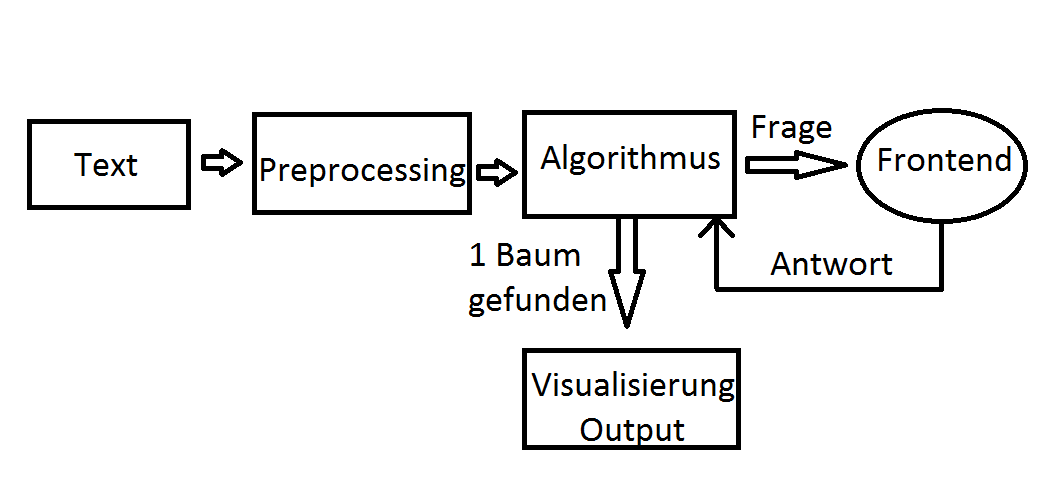
\includegraphics[scale=0.4]{Grafik}
 \end{center}
Das System besteht bekanntlich aus drei Teilbereichen, die durch Schnittstellen kommunizieren:
\begin{itemize}
\item Preprocessing\\Generieren der möglichen Parsebäume und Übergabe der $k$-besten an die Fragengenerierung über die Schnittstelle Preprocessing - Fragegenerierung
\item Algorithmus zur Fragengenerierung auf einem Server\\erhält die $k$-besten Parsebäume 
\item Client\\Übermittlung der
Fragen an den Annotator und der Antwort des Annotators an den Algorithmus über die Schnittstelle Client - Server sowie vom Prozess unabhängige Darstellung des Parsebaums 
\end{itemize}

\subsection{AaS-Server}
\label{sub:AaS-Server}
Der AaS-Server generiet die Fragen, nach welchen der optimale Parsebaum ausgeählt wird. Der Algorithmus folgt dabei folgendem Schema:
    \begin{itemize}
        \item Generiere aus Parseforest die Frage, welche bei ihrer Beantwortung die meisten Bäume rausfiltert.
            \begin{itemize}
                \item Suche des Tupels, das den Suchraum am ehesten halbiert:
            \end{itemize}
    \end{itemize}

        \indent\indent\indent\indent\indent\indent a $\gets$ len(parses) Anzahl der Parse-Bäume. \\
        \indent\indent\indent\indent\indent\indent For each tuple \\
       \indent\indent\indent\indent\indent\indent\indent score $\gets$ $\mathrm{abs}(\mathrm{count(tuple)} - \frac{a}{2})$ \\
        \indent\indent\indent\indent\indent\indent End For

    \begin{itemize}
        \item Nimm den Tupel als Frage
    \end{itemize}
Näheres im AaSP.

\subsubsection{Dependencies}
\label{ssub:Server-Dependencies}
Der Algorithmus benötigt folgende Software um korrekt zu laufen:
    \begin{itemize}
        \item Python $\geq$ 3.4 
        \item Python3 packages: asyncio, Flask
        \item Parser, der k-best Parses liefert (Anders Bjorkelunds transition-based parser )
        \item TCP- oder UNIX-Sockets
        \item JSON
    \end{itemize}

\subsubsection{Algorithm}
\label{ssub:Algorithm}

\subsection{AaS-CLI-Client}
\label{sub:AaS-CLI-Client}

\subsubsection{Dependencies}
\label{ssub:CLI-Client-Dependencies}

\subsection{AaS-Web-Client}
\label{sub:AaS-Web-Client}

\subsubsection{Dependencies}
\label{ssub:Web-Client-Dependencies}

\end{document}
